\documentclass[11pt,a4paper]{article}

\usepackage[a4paper,margin=2.2cm]{geometry}
\usepackage{booktabs}
\usepackage{multirow}
\usepackage{graphicx}
\usepackage{subcaption}
\usepackage{amsmath,amssymb}
\usepackage{siunitx}
\usepackage[hidelinks]{hyperref}
\usepackage{xcolor}
\usepackage{caption}
\usepackage{float}
\usepackage{microtype}
\usepackage{setspace}
\setstretch{1.02}

\definecolor{mpcblue}{HTML}{1D4ED8}
\newcommand{\mpcbest}[1]{\textcolor{mpcblue}{\textbf{#1}}}

\captionsetup{font=small,labelfont=bf}
\captionsetup[sub]{font=scriptsize,labelfont=bf}
\setlength{\floatsep}{8pt plus 2pt minus 2pt}
\setlength{\textfloatsep}{10pt plus 2pt minus 2pt}
\setlength{\intextsep}{8pt plus 2pt minus 2pt}
\setlength{\abovecaptionskip}{4pt}
\setlength{\belowcaptionskip}{2pt}

\title{%
  Offset-Free Model Predictive Control for an Industrial DC Motor Drive:\\
  Comparison with Hand-Tuned and Optimised PID}
\author{%
  Vinayak Raizada, Vansh Gautam, Vrinda Gupta, Sushant Goyal\\
  Department of Electrical Engineering, IIT Roorkee}
\date{}

\begin{document}
\maketitle
\thispagestyle{empty}

\begin{abstract}
Model predictive control (MPC) plans the next actuator move by rolling a plant model forward over a finite horizon and solving a constrained optimisation at every sample.
We build an offset-free MPC for the speed of a permanent-magnet DC (PMDC) motor, and compare it with a hand-tuned PID and an optimised PID on ten reproducible scenarios.
All three controllers command the armature voltage through the same simulated drive, which saturates the voltage, limits its slew rate, and protects against over-current, and they face identical references, load torques and noise.
The MPC predicts armature current and speed, respects voltage, voltage-rate and current constraints, and estimates both the load torque and an armature-voltage disturbance so that it stays offset-free under resistance mismatch.
Optimised PID gains are found once on a speed-tracking scenario and then frozen.
MPC has the lowest speed-tracking error and the fastest settling in most scenarios, including startup, tracking, load changes, encoder noise, reversal and plant mismatch, and the lowest time spent in current limit under current protection.
Where the drive limits dominate, the three controllers are close.
The MPC also uses the measured current, which the PID loops do not, and all parameters are illustrative.
\end{abstract}

\begin{figure}[H]
  \centering
  \includegraphics[width=0.92\textwidth]{figures/mpc-infographic.png}
  \caption{MPC loop: predict states and inputs over a horizon, apply the first move to the plant, and close the loop with measured feedback and disturbance \(\theta(t)\).}
  \label{fig:mpc-loop}
\end{figure}

\section{Introduction}
A PMDC motor with controlled armature voltage is a standard industrial drive: it turns conveyors, pumps, machine axes and material-handling equipment.
The control task is to hold a shaft speed while the load changes, the supply wobbles and the encoder is noisy, without asking the drive for more voltage, voltage slew or current than it may deliver.
A PID loop reacts only after the speed has already moved, and a limit applied after the fact does not undo the mistake that the controller made while it did not know about the limit.
MPC uses a model to predict the response to different voltage choices, re-solves every sample (receding horizon), and can enforce voltage, rate and current limits inside the optimiser~\cite{rawlings2017,camacho2013}.
Figure~\ref{fig:mpc-loop} shows the idea.

We implement it with a two-state linear prediction model, a disturbance estimate for offset-free tracking~\cite{pannocchia2003}, a constrained quadratic programme solved with SLSQP, and a simulated motor as the truth plant.
All motor numbers are illustrative, not data from a commercial motor.

\section{Background and models}
We keep four models separate: the actual plant, the controller's prediction model, the drive, and the measurement model.

\subsection{Actual plant}
The plant is the coupled electrical and mechanical system
\begin{equation}
  L_a \frac{di_a}{dt} = V_a - R_a i_a - K_e\omega,\qquad
  J\frac{d\omega}{dt} = K_t i_a - B\omega - T_L,\qquad
  \frac{d\theta}{dt}=\omega,
  \label{eq:motor}
\end{equation}
with \(R_a{=}1.0\,\si{\ohm}\), \(L_a{=}10\,\si{\milli\henry}\), \(K_t{=}K_e{=}0.05\), \(J{=}0.002\,\si{\kilogram\meter\squared}\), \(B{=}0.001\,\si{\newton\meter\second}\), nominal load \(T_L{=}0.05\,\si{\newton\meter}\), \(V_{\max}{=}24\,\si{\volt}\), \(I_{\max}{=}8\,\si{\ampere}\).
In state-space form with \(x=[i_a,\omega,\theta]^\top\), \(A=\bigl[\begin{smallmatrix}-100&-5&0\\25&-0.5&0\\0&1&0\end{smallmatrix}\bigr]\), \(B=[100,0,0]^\top\), \(E=[0,-500,0]^\top\), and the poles lie at \(-98.7\) and \(-1.75\,\si{\per\second}\): an electrical time constant of \(10\,\si{\milli\second}\) and a mechanical one of about \(0.57\,\si{\second}\).
The plant is integrated with fixed-step RK4 at \(1\,\si{\milli\second}\) while the controller runs every \(10\,\si{\milli\second}\) with its output held; a \(10\,\si{\milli\second}\) integration step would not resolve the electrical mode.

\subsection{Prediction model and observer}
MPC predicts with the \(2\)-state model \(x_{k+1}=A_dx_k+B_d(V_k+\hat d_V)+E_d\hat d_T\), \(x=[i_a,\omega]^\top\), obtained by exact zero-order-hold discretisation of the nominal motor.
Each sample the innovations of the measured current and speed are mapped back to two disturbance estimates through \([B_d\;E_d]\), scaled by an observer gain \(g{=}0.1\).
The torque estimate \(\hat d_T\) absorbs load and friction error; the voltage estimate \(\hat d_V\) absorbs electrical error such as a wrong resistance.
A torque-only estimate left a speed offset of about \(44\,\mathrm{RPM}\) under \(+20\%\) resistance in development, which estimating both removed~\cite{pannocchia2003}.

\subsection{Drive}
Every command passes through one drive: enable and latched emergency stop, a slew limit (\(1200\,\si{\volt\per\second}\)), saturation at \(\pm V_{\max}\) times the DC-bus level, and current protection.
Protection is a voltage window that keeps the exact one-sample electrical response inside \(\pm I_{\max}\), computed from the drive's nominal \(R_a,K_e\) and the measured current and speed, with a feedback term on measured excess current; it is not a clip of the simulated state.

\subsection{Measurement}
Speed comes from an encoder with seeded Gaussian noise; current is measured ideally.

\section{Controllers}
\subsection{MPC}
Over \(N{=}60\) samples (\(0.6\,\si{\second}\)) the controller chooses \(n_u{=}6\) voltage moves with block lengths \(1,2,4,\dots\) samples and minimises
\begin{equation}
  J = q\sum_{k=1}^{N}(\omega_k-r_k)^2 + q_T(\omega_N-r_N)^2 + r_\Delta\sum_j\Delta V_j^2,
  \label{eq:cost}
\end{equation}
in \(\mathrm{RPM}^2\) and \(\si{\volt\squared}\), with reference preview \(r_k\), \(q{=}1\), \(q_T{=}50\), \(r_\Delta{=}5000\).
Constraints are the voltage box, the voltage change between moves, and the predicted armature current \(|i_{a,k}|\le I_{\max}\) over the whole horizon.
All are linear in the decision variables, so SLSQP receives analytic gradients; solves take about \(1\)--\(5\,\si{\milli\second}\).

\subsection{PID baselines}
The positional PID takes RPM and returns volts, with a filtered derivative on the measurement and back-calculation anti-windup against the voltage the drive \emph{actually applied}, so slew, saturation and current limiting all unwind the integrator.
Hand-tuned gains (\(K_p{=}0.01\), \(K_i{=}0.03\), \(K_d{=}0\)) are a deliberately conservative guess.
Optimised gains minimise a dimensionless sum of IAE, overshoot, settling time, voltage effort, time in voltage saturation and time in current limit with L-BFGS-B~\cite{astrom2006}.
They are found once on the speed-tracking scenario (\(K_p{=}0.0326\), \(K_i{=}0.131\), \(K_d{=}0\)) and frozen for all comparisons.

\section{System design and implementation}
\label{sec:design}
Figure~\ref{fig:arch} shows the closed loop.
All controllers drive the same plant through the same drive and are scored with the same metrics.

\begin{figure}[H]
  \centering
  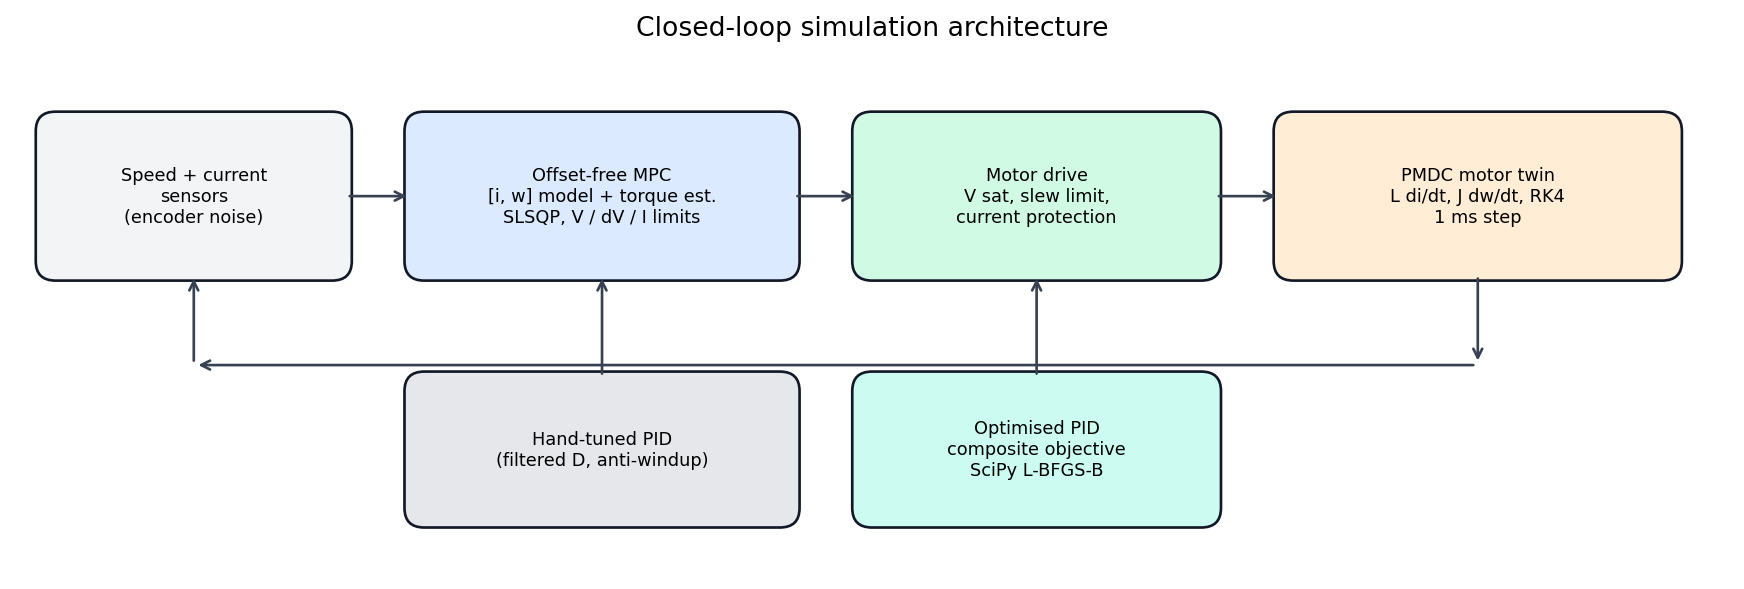
\includegraphics[width=0.95\textwidth]{figures/architecture.png}
  \caption{Simulation architecture: offset-free MPC and both PID variants act on one motor through one drive.}
  \label{fig:arch}
\end{figure}

\section{Experimental setup}
Controller sample \(10\,\si{\milli\second}\), plant step \(1\,\si{\milli\second}\), nominal load \(0.05\,\si{\newton\meter}\).
The ten scenarios, each reproducible (seeded noise, identical arrays for every controller), are:
\begin{enumerate}
  \item \textbf{Motor startup:} \(0\to1000\,\mathrm{RPM}\) at nominal load.
  \item \textbf{Speed tracking:} \(1000/2000/1500/2500\,\mathrm{RPM}\), \(5\,\si{\second}\) each.
  \item \textbf{Sudden load:} at \(2000\,\mathrm{RPM}\), load \(0.05\to0.10\,\si{\newton\meter}\) at \(5\,\si{\second}\).
  \item \textbf{Load removal:} \(0.10\to0.05\,\si{\newton\meter}\) at \(5\,\si{\second}\).
  \item \textbf{Voltage saturation:} \(2900\,\mathrm{RPM}\) reference, DC bus sags to \(85\%\) at \(8\,\si{\second}\).
  \item \textbf{Current protection:} \(2500\,\mathrm{RPM}\), load rises to \(0.14\,\si{\newton\meter}\), which needs more than \(8\,\si{\ampere}\) to hold speed.
  \item \textbf{Model mismatch:} plant \(R_a{+}20\%\), \(J{+}30\%\), \(B{+}25\%\) (and the opposite corner), load step at \(8\,\si{\second}\); controllers keep the nominal model.
  \item \textbf{Sensor noise:} \(15\,\mathrm{RPM}\) encoder noise during a \(1000\to1500\,\mathrm{RPM}\) step.
  \item \textbf{Variable load:} \(0.5\,\si{\hertz}\) sinusoid plus bounded random torque at \(1500\,\mathrm{RPM}\).
  \item \textbf{Reverse operation:} \(+1000\to-1000\to+1000\,\mathrm{RPM}\).
\end{enumerate}
Settling uses a \(2\%\) band on the last reference segment; IAE is in \(\mathrm{RPM\,s}\).

\section{Results}
Blue bold cells mark where MPC is lowest (or tied lowest) among the three controllers on settling time, overshoot or IAE; black bold marks a PID variant that is lowest or tied.
Peak current and time in current limit are shown for context, not ranked.
All numbers are generated by \texttt{scripts/rebuild\_report\_metrics.py} from the code in this repository.

\begin{table}[H]
\centering
\scriptsize
\caption{Closed-loop metrics for the ten scenarios (plus the opposite mismatch corner). Optimised PID uses the frozen gains.}
\label{tab:summary}
\begin{tabular}{@{}llrrrrr@{}}
\toprule
Scenario & Controller & Settling [s] & Overshoot [\%] & IAE [RPM s] & Peak I [A] & Current-limited [s] \\
\midrule
\multirow{3}{*}{Motor startup} & MPC & \mpcbest{0.76} & \mpcbest{0.0} & \mpcbest{351} & 7.98 & 0.60 \\
 & PID & 1.84 & 2.8 & 414 & 7.97 & 0.20 \\
 & Opt. PID & 0.92 & 0.2 & 364 & 7.99 & 0.45 \\
\midrule
\multirow{3}{*}{Speed-reference tracking} & MPC & \mpcbest{0.87} & \mpcbest{0.0} & \mpcbest{1071} & 7.99 & 3.05 \\
 & PID & 1.58 & 1.0 & 1854 & 7.99 & 1.81 \\
 & Opt. PID & 1.49 & 0.1 & 1660 & 7.99 & 2.65 \\
\midrule
\multirow{3}{*}{Sudden mechanical load} & MPC & \mpcbest{0.00} & \mpcbest{0.0} & \mpcbest{3} & 6.42 & 0.00 \\
 & PID & \textbf{0.00} & \textbf{0.0} & 35 & 6.33 & 0.00 \\
 & Opt. PID & \textbf{0.00} & \textbf{0.0} & 8 & 6.35 & 0.00 \\
\midrule
\multirow{3}{*}{Load removal} & MPC & \mpcbest{0.00} & \mpcbest{0.0} & \mpcbest{3} & 6.19 & 0.00 \\
 & PID & \textbf{0.00} & \textbf{0.0} & 35 & 6.19 & 0.00 \\
 & Opt. PID & \textbf{0.00} & \textbf{0.0} & 8 & 6.19 & 0.00 \\
\midrule
\multirow{3}{*}{Voltage saturation} & MPC & — & \mpcbest{0.0} & \mpcbest{3307} & 8.00 & 3.84 \\
 & PID & — & 0.3 & 4122 & 7.99 & 3.00 \\
 & Opt. PID & — & \textbf{0.0} & 4092 & 8.00 & 3.53 \\
\midrule
\multirow{3}{*}{Current protection} & MPC & \mpcbest{3.89} & \mpcbest{0.0} & \mpcbest{3626} & 8.00 & 4.34 \\
 & PID & 3.92 & 0.2 & 3678 & 8.00 & 9.18 \\
 & Opt. PID & \textbf{3.89} & \textbf{0.0} & 3635 & 8.00 & 9.71 \\
\midrule
\multirow{3}{*}{Model mismatch} & MPC & \mpcbest{2.08} & \mpcbest{0.3} & \mpcbest{1290} & 7.14 & 4.47 \\
 & PID & 2.69 & 1.4 & 1794 & 7.23 & 4.10 \\
 & Opt. PID & 2.67 & 0.4 & 1700 & 7.36 & 4.25 \\
\midrule
\multirow{3}{*}{Sensor noise} & MPC & \mpcbest{0.25} & 2.3 & \mpcbest{103} & 7.98 & 0.16 \\
 & PID & 0.68 & 5.0 & 181 & 7.98 & 0.08 \\
 & Opt. PID & 0.63 & \textbf{1.8} & 160 & 7.99 & 0.22 \\
\midrule
\multirow{3}{*}{Variable load} & MPC & \mpcbest{0.00} & \mpcbest{0.0} & \mpcbest{45} & 5.48 & 0.00 \\
 & PID & 11.74 & \textbf{0.0} & 275 & 5.32 & 0.00 \\
 & Opt. PID & \textbf{0.00} & \textbf{0.0} & 96 & 5.50 & 0.00 \\
\midrule
\multirow{3}{*}{Reverse operation} & MPC & \mpcbest{0.69} & \mpcbest{0.0} & \mpcbest{1132} & 7.98 & 1.62 \\
 & PID & 2.37 & 1.4 & 2199 & 7.97 & 1.10 \\
 & Opt. PID & 1.44 & 0.1 & 2079 & 7.97 & 1.65 \\
\midrule
\multirow{3}{*}{Model mismatch (low R, J, B)} & MPC & \mpcbest{0.33} & \mpcbest{0.0} & \mpcbest{468} & 8.98 & 0.39 \\
 & PID & 1.17 & \textbf{0.0} & 756 & 9.10 & 0.25 \\
 & Opt. PID & 0.87 & \textbf{0.0} & 615 & 9.10 & 0.50 \\
\bottomrule
\end{tabular}

\end{table}

Figure~\ref{fig:iae} summarises IAE and Figure~\ref{fig:traces} shows four responses.

\begin{figure}[H]
  \centering
  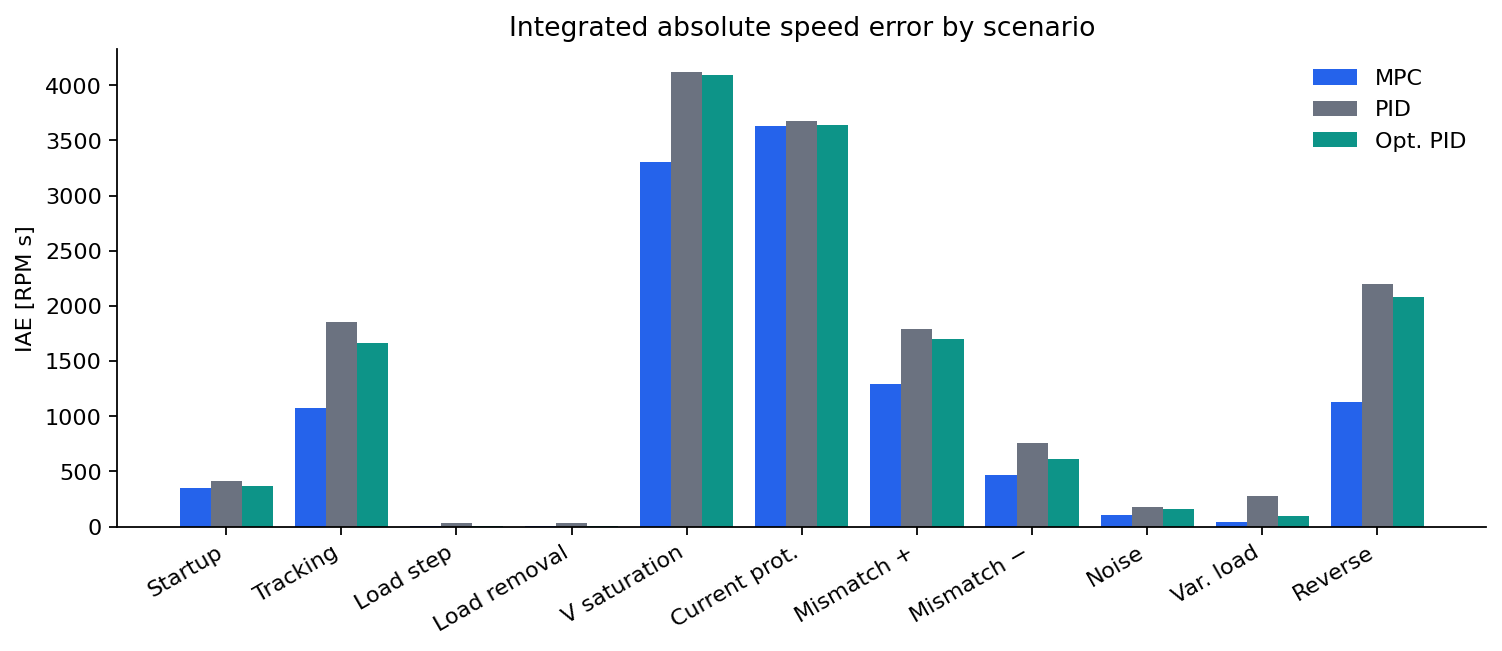
\includegraphics[width=0.95\textwidth]{figures/iae_bars.png}
  \caption{IAE by scenario.}
  \label{fig:iae}
\end{figure}

\begin{figure}[H]
  \centering
  \begin{subfigure}[t]{0.48\textwidth}
    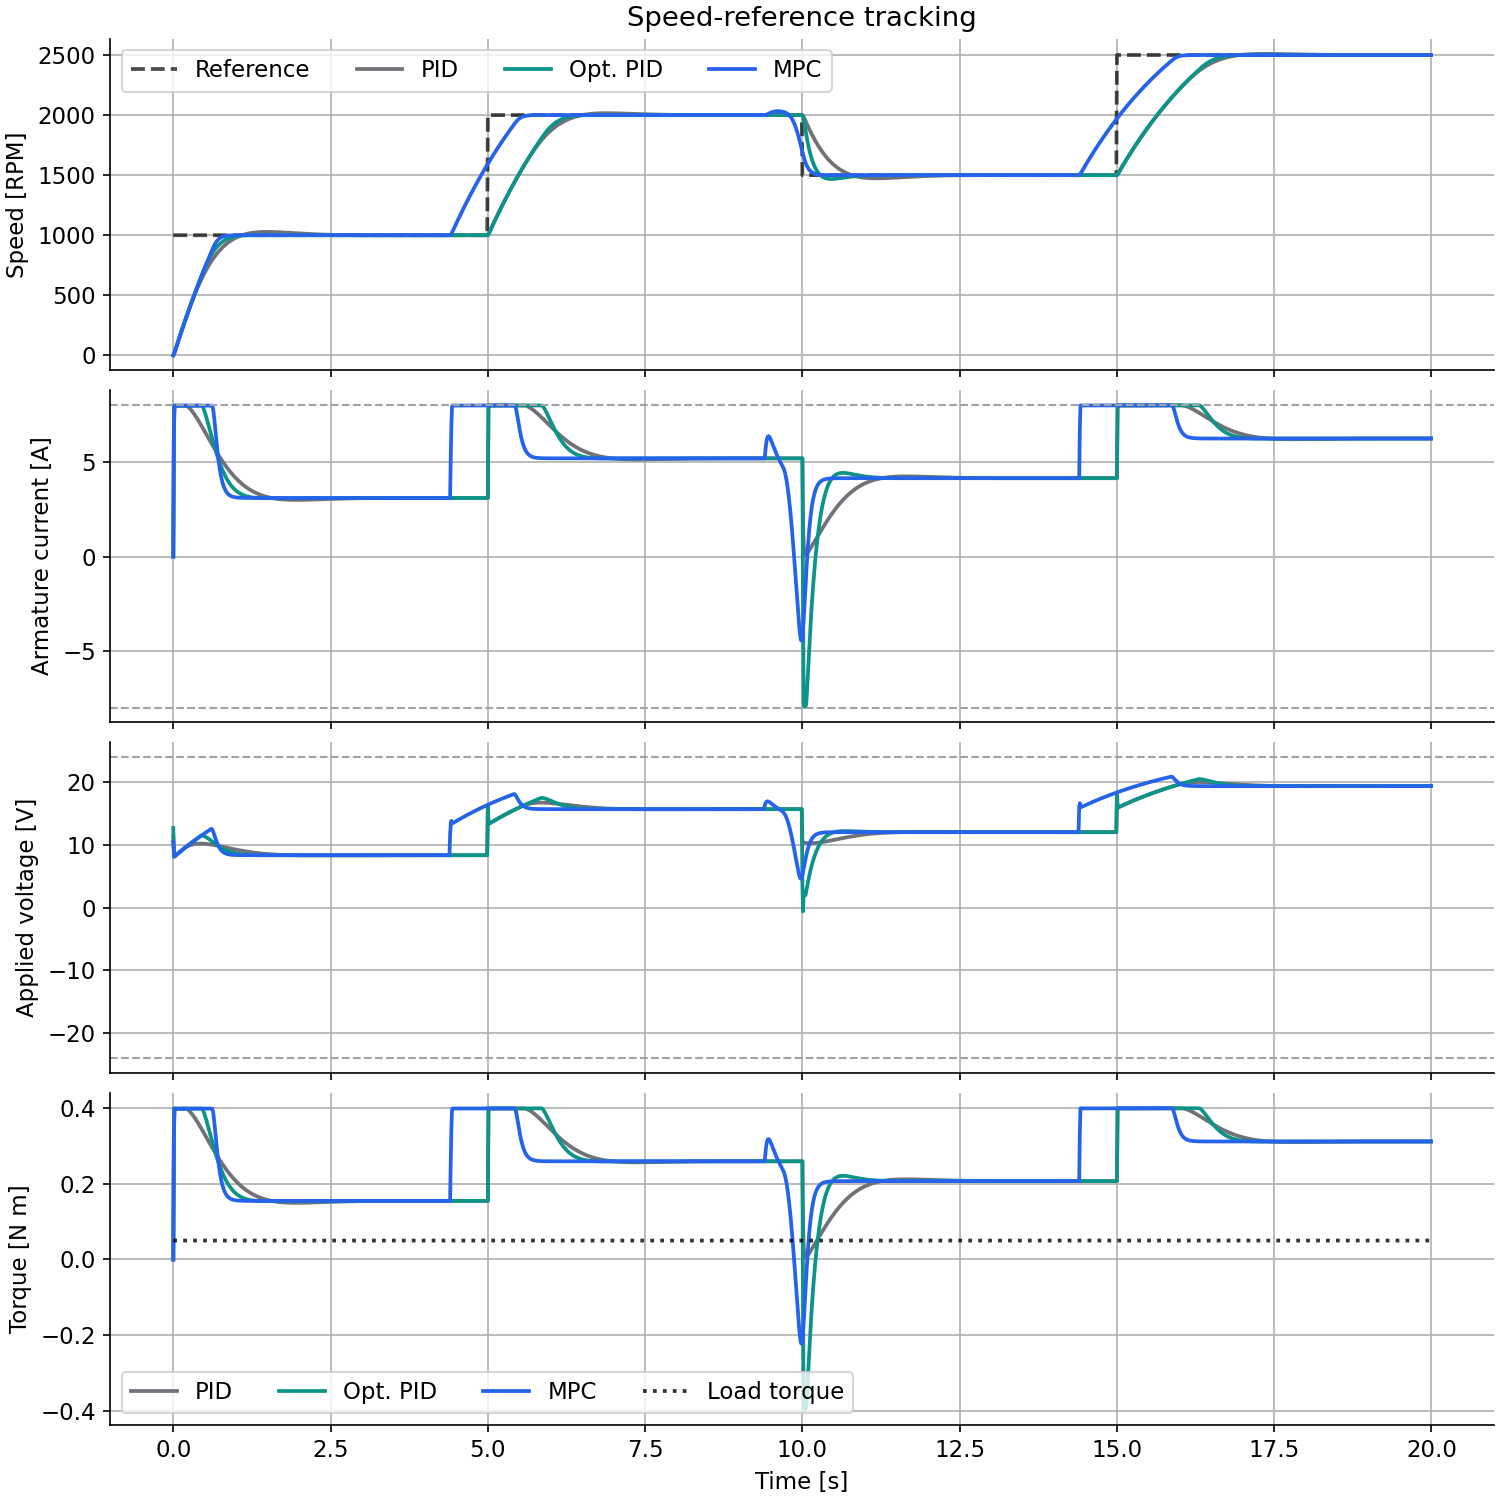
\includegraphics[width=\linewidth]{figures/speed_tracking.png}
    \caption{Speed tracking}
  \end{subfigure}\hfill
  \begin{subfigure}[t]{0.48\textwidth}
    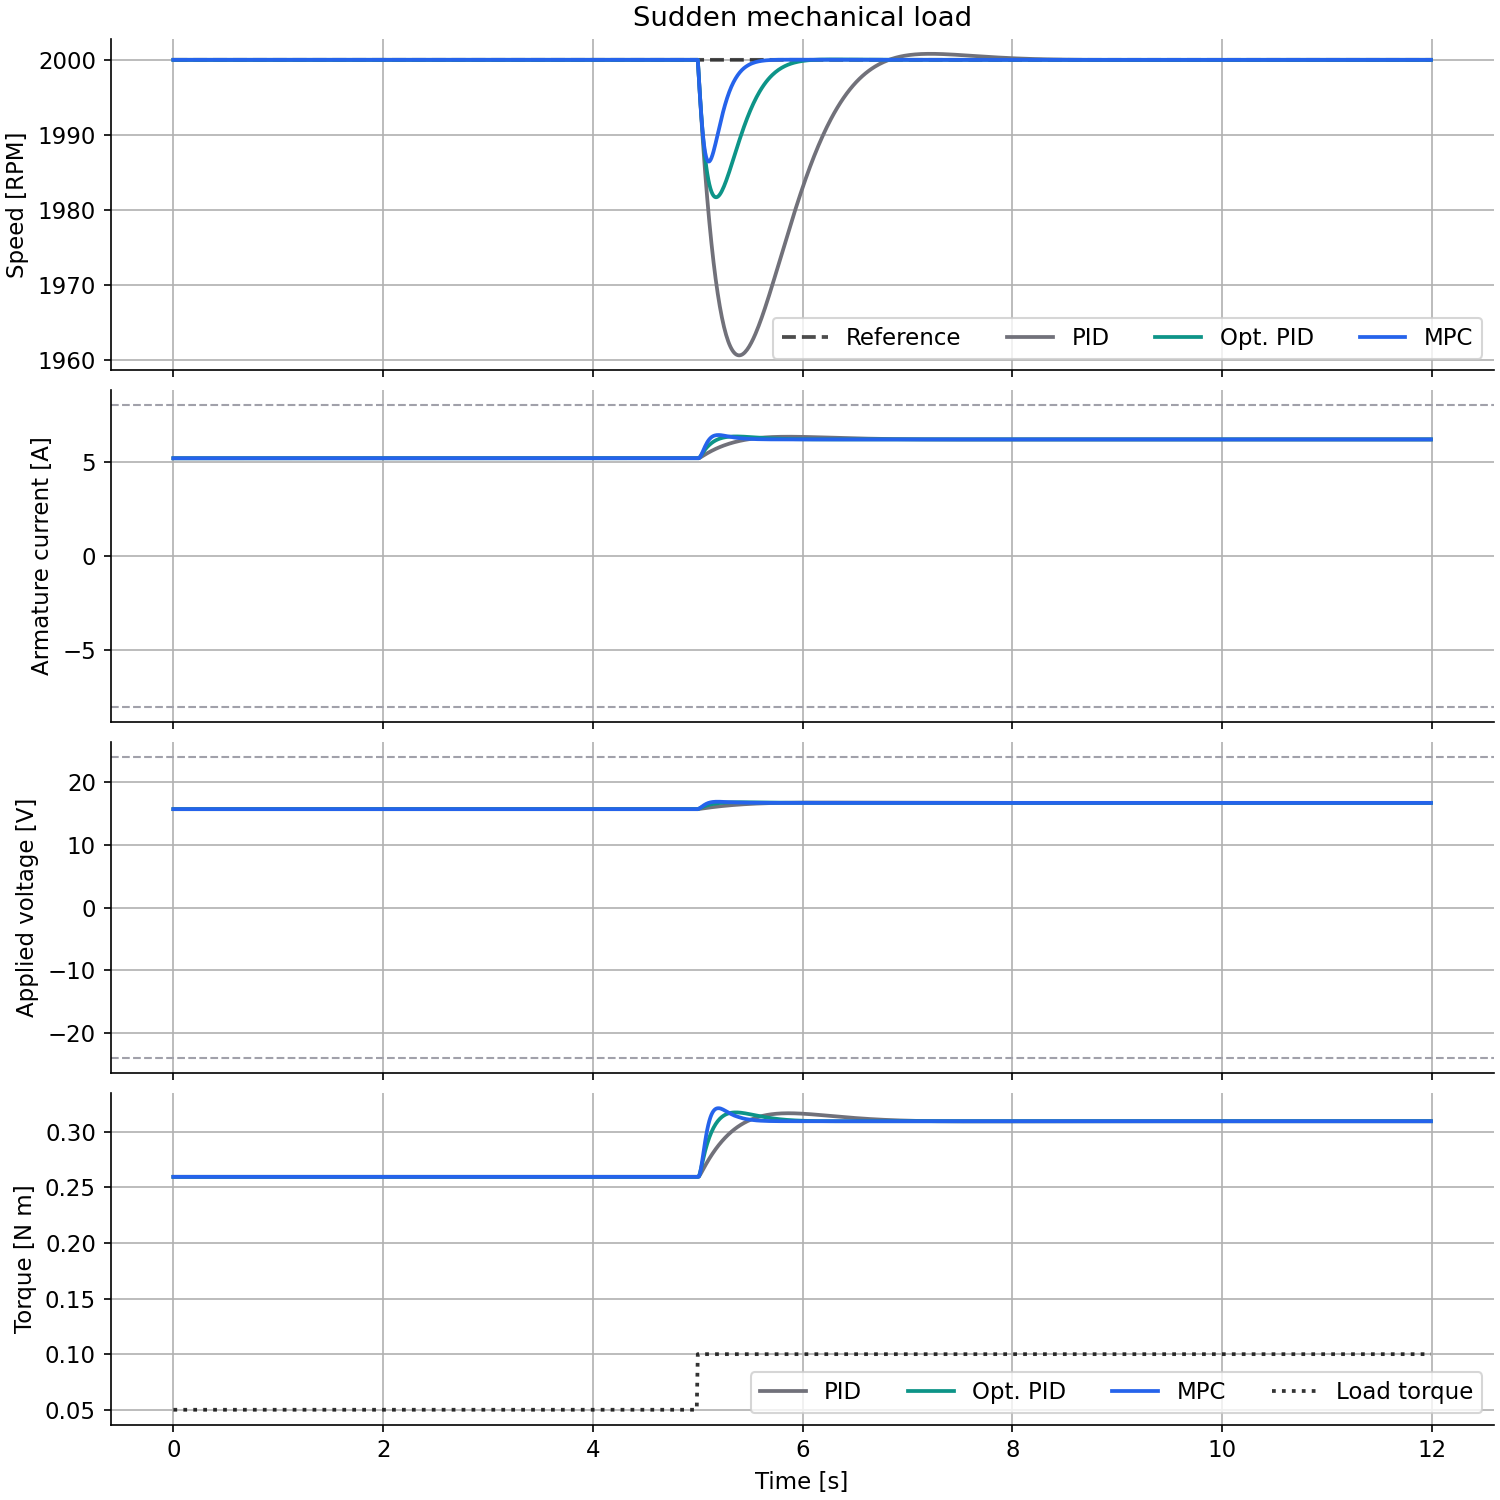
\includegraphics[width=\linewidth]{figures/load_step.png}
    \caption{Sudden load}
  \end{subfigure}

  \vspace{0.35em}
  \begin{subfigure}[t]{0.48\textwidth}
    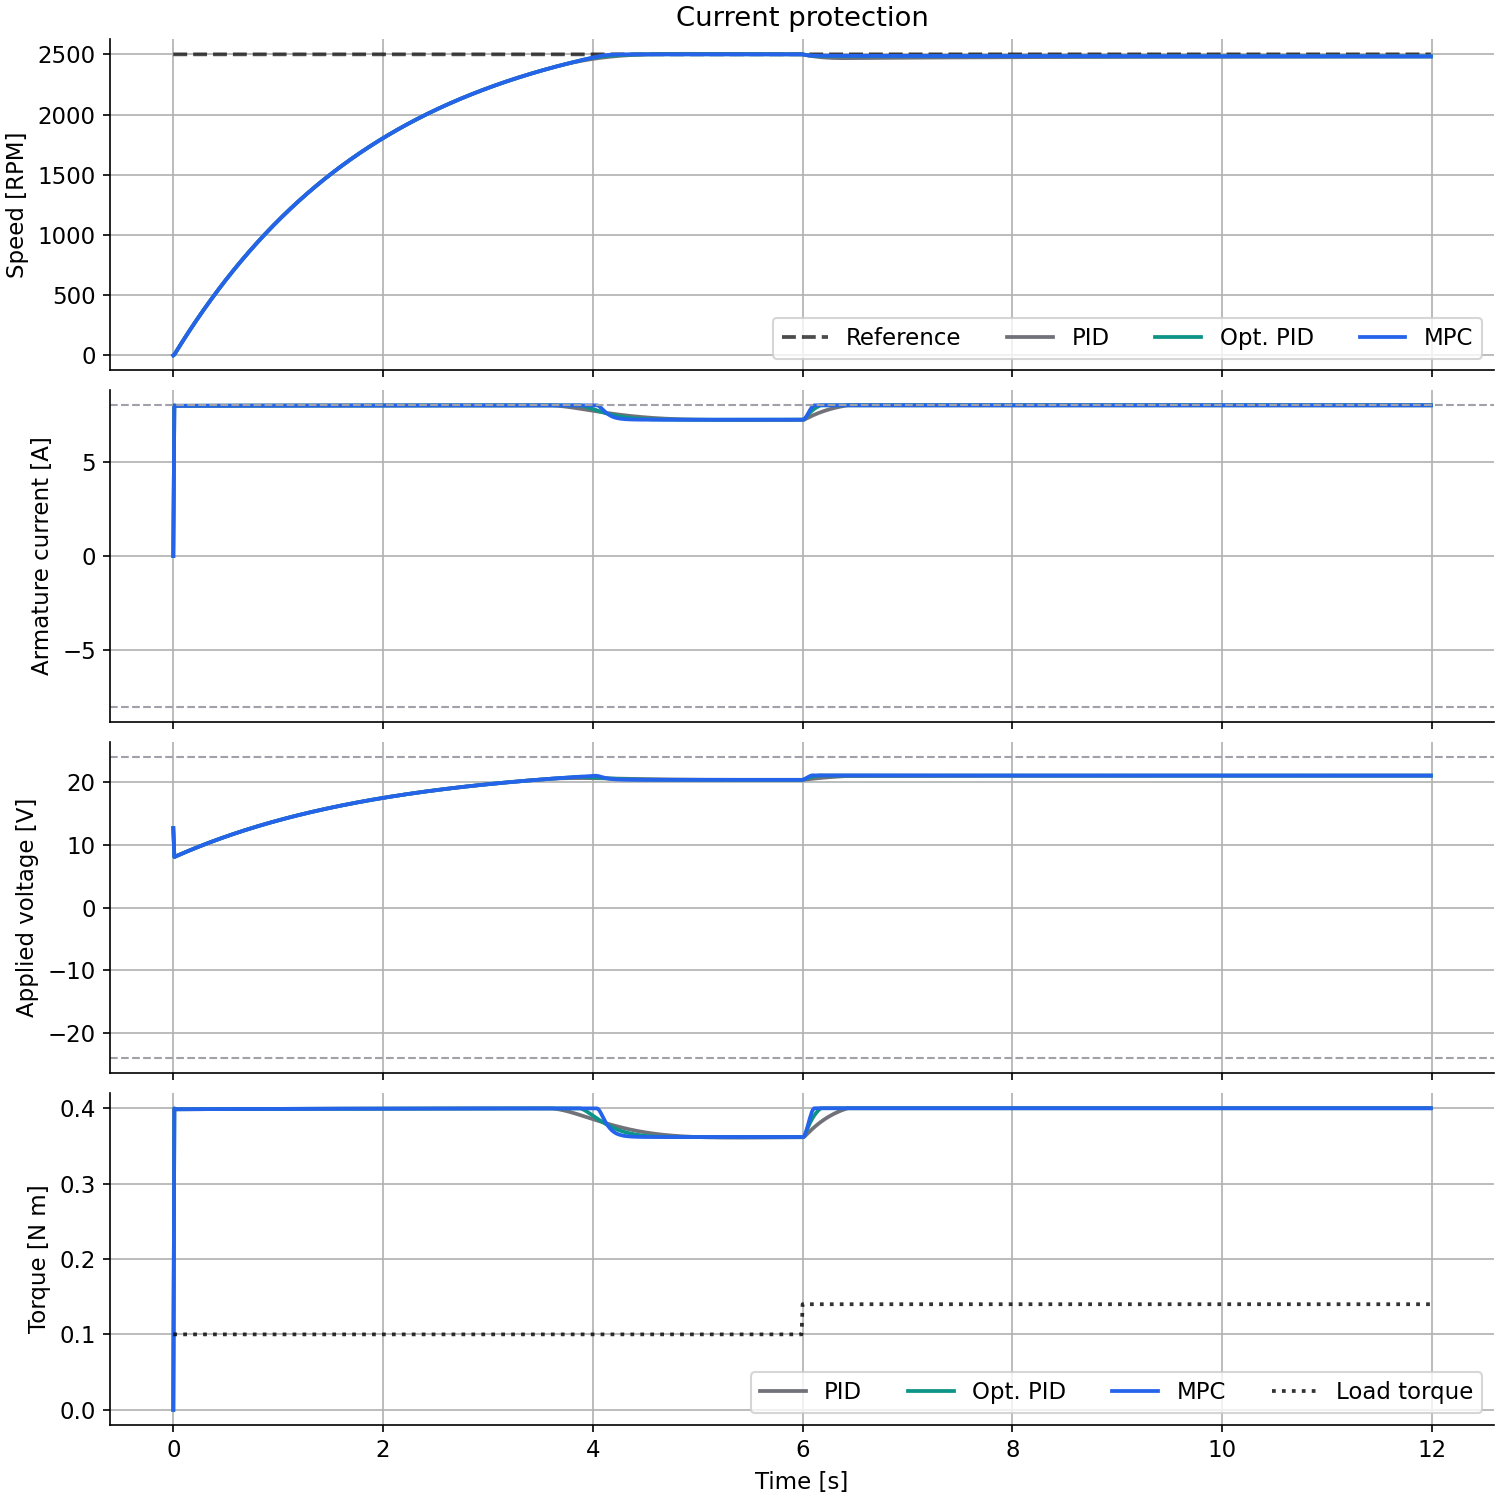
\includegraphics[width=\linewidth]{figures/current_protection.png}
    \caption{Current protection}
  \end{subfigure}\hfill
  \begin{subfigure}[t]{0.48\textwidth}
    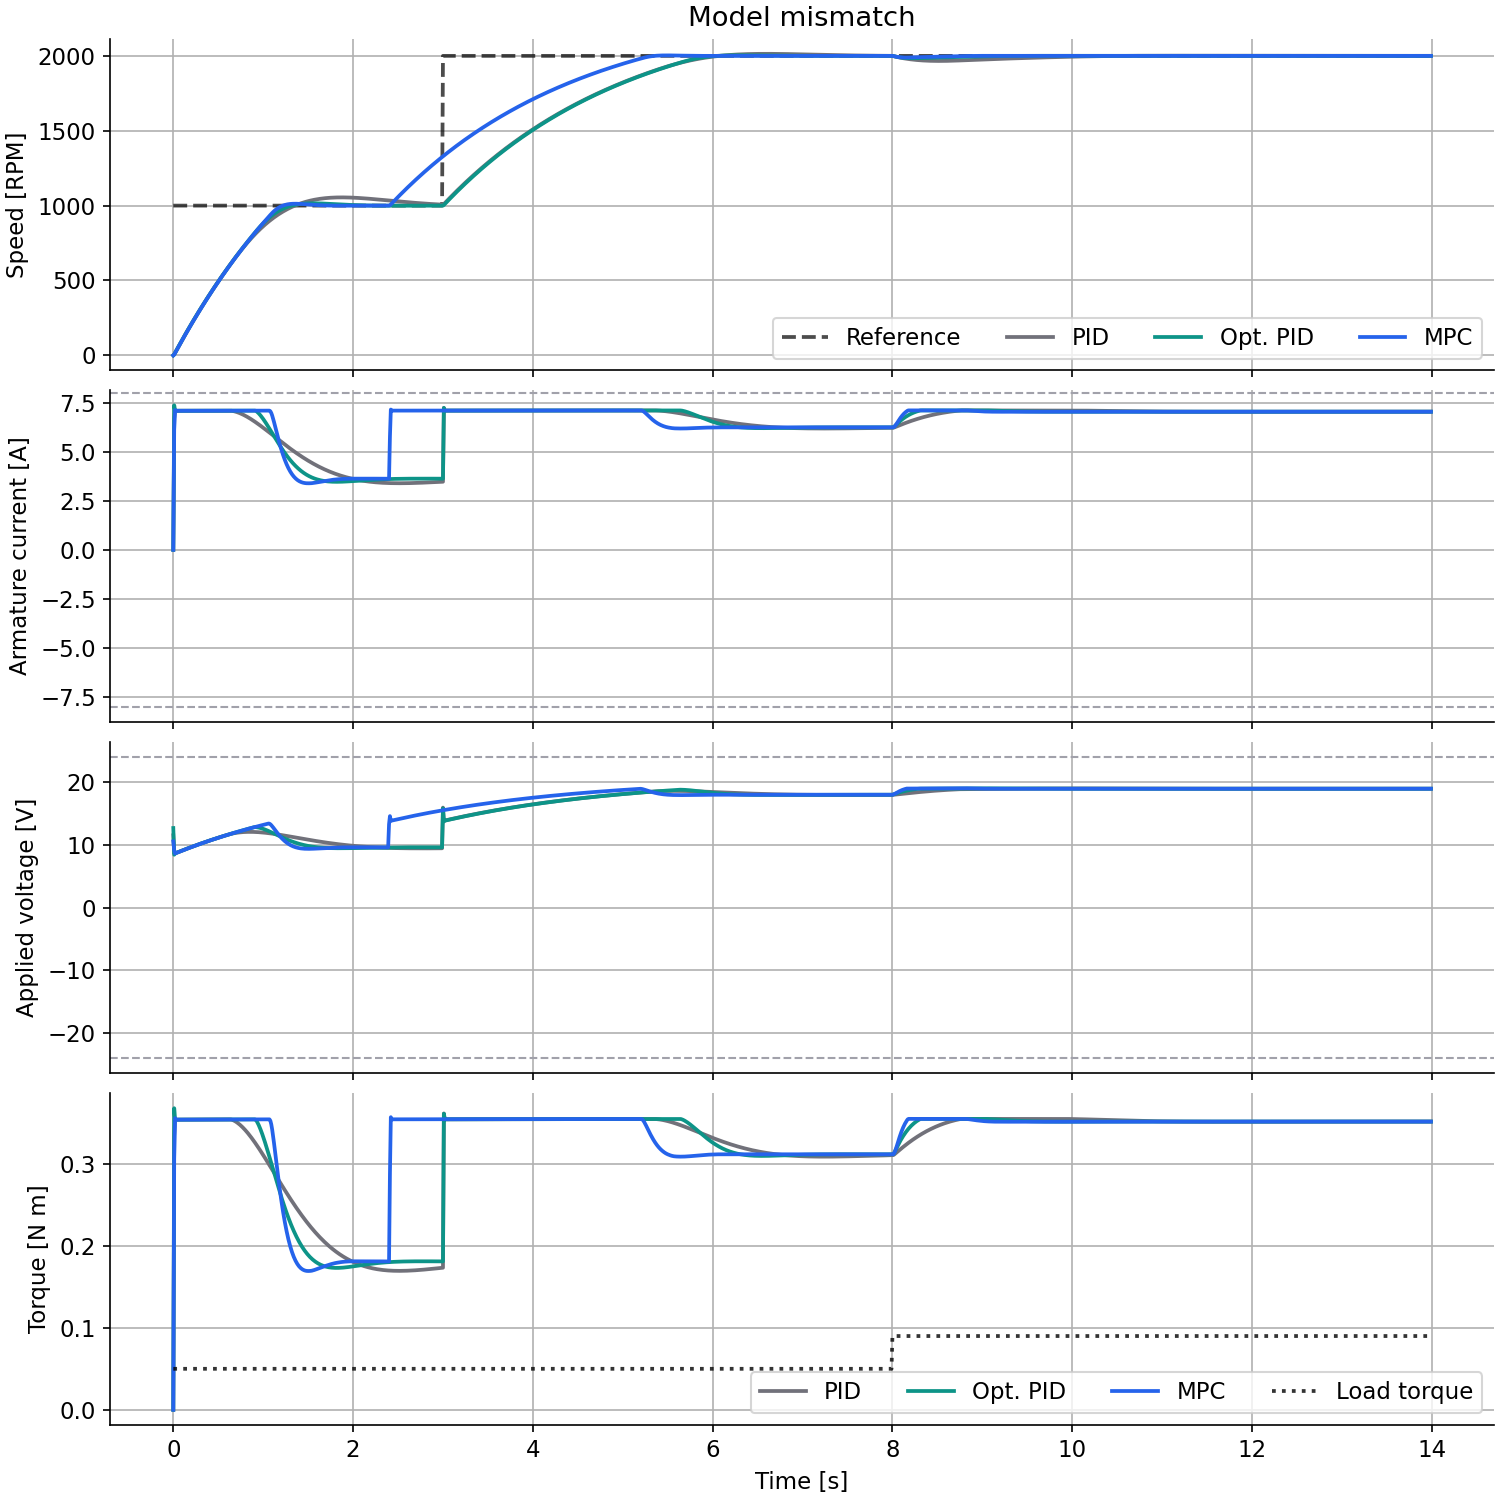
\includegraphics[width=\linewidth]{figures/model_mismatch.png}
    \caption{Model mismatch}
  \end{subfigure}
  \caption{Speed, armature current, voltage and torque for MPC, PID and optimised PID.}
  \label{fig:traces}
\end{figure}

\subsection{Tracking and load changes}
MPC settles startup in \(0.76\,\si{\second}\) against \(1.84\,\si{\second}\) for the hand-tuned PID and \(0.92\,\si{\second}\) for the optimised PID, and has the lowest IAE on speed tracking (\(1071\) against \(1854\) and \(1660\)).
Much of the gap on the load step (IAE \(3\) against \(35\) and \(8\)) and the variable load is the disturbance estimator reacting within a sample or two; a PID with a larger integral gain could narrow it, at the cost of noise sensitivity.

\subsection{Drive limits}
In the voltage-saturation and current-protection scenarios the actuator, not the algorithm, sets the best achievable response, and the controllers end up close (current-protection IAE \(3626\) against \(3678\) and \(3635\)).
MPC does keep the drive out of its current limit for less time (\(4.34\,\si{\second}\) against \(9.18\) and \(9.71\)), because it plans along the \(8\,\si{\ampere}\) bound instead of running into it.
Under \(\pm20\%\) resistance error the drive's current limit can be exceeded transiently, up to \(9.1\,\si{\ampere}\) against an \(8\,\si{\ampere}\) limit in the low-resistance corner, before the feedback term backs off.

\begin{figure}[H]
  \centering
  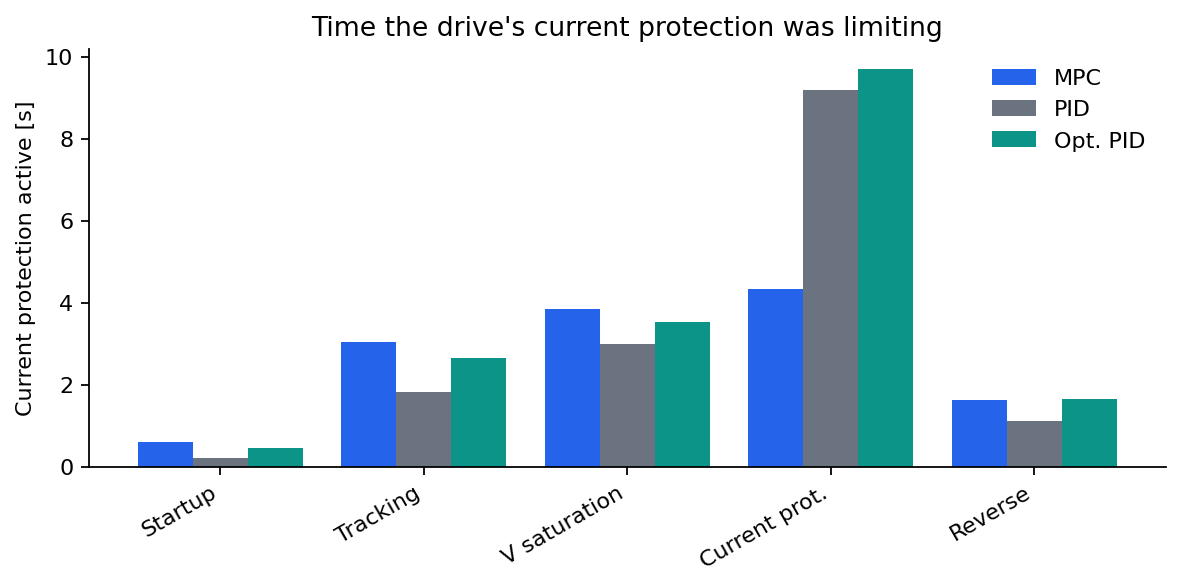
\includegraphics[width=0.72\textwidth]{figures/current_limit_bars.png}
  \caption{Time the drive's current protection was limiting, in the scenarios that reach the limit.}
  \label{fig:ilim}
\end{figure}

\subsection{Noise and robustness}
With \(15\,\mathrm{RPM}\) encoder noise the MPC keeps the lowest IAE (\(103\) against \(181\) and \(160\)), after the observer gain was lowered to \(0.1\); at gain \(1\) it amplified the noise into the voltage and lost to the PID.
Under plant mismatch the MPC stays offset-free and has IAE \(1290\) against \(1700\) for the frozen optimised PID and \(1706\) for a PID retuned on the mismatched plant (Figure~\ref{fig:rob}).

\begin{figure}[H]
  \centering
  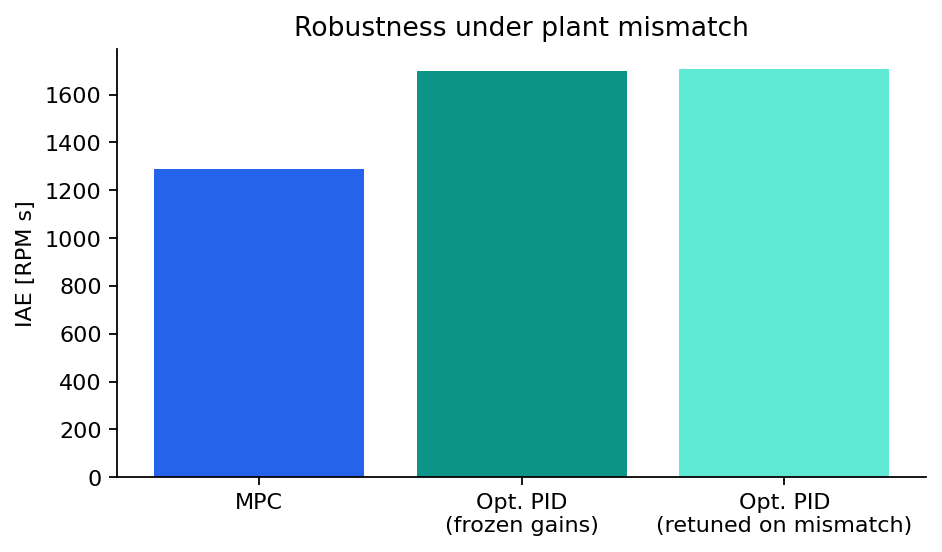
\includegraphics[width=0.88\textwidth]{figures/robustness_bars.png}
  \caption{IAE under plant mismatch: MPC, frozen optimised PID, and optimised PID retuned on the mismatched plant.}
  \label{fig:rob}
\end{figure}

\section{Discussion and limitations}
Offset-free MPC is the better controller here, but the comparison favours it in three ways: it uses the measured current and a nominal model that matches the plant when no mismatch is applied, the PID loops are single-loop speed controllers, and its weights, horizon and observer gain are hand-set after looking at these scenarios.
The optimised PID is tuned on one scenario, so its advantage elsewhere is whatever carries over, which is the point of freezing it; retuning on the mismatched plant did not help it.

The model is linear with constant parameters.
It omits brush drop, magnetic saturation, temperature dependence of the resistance, Coulomb friction and shaft compliance; the load torque keeps its sign at standstill; the current sensor is ideal; and the converter efficiency (\(0.95\)) is illustrative, so the drive and motor efficiency figures in the repository (about \(0.1\)--\(0.2\), dominated by copper loss at these small shaft powers) are not data.
No stability proof is claimed for the MPC, and the solve time of a few milliseconds is not a hard real-time guarantee.

\section{Conclusion}
For this PMDC motor drive, offset-free MPC with reference preview is the controller to prefer when constraints and disturbances matter: it leads on startup, tracking, load changes, noise, reversal and mismatch, plans along the current limit instead of hitting it, and does not need retuning when the load or plant change.
Where the drive's limits decide the outcome, the controllers are close, and a well-tuned PID remains a reasonable choice.

\begin{thebibliography}{4}
\footnotesize
\bibitem{pannocchia2003}
G.~Pannocchia and J.~B.~Rawlings,
``Disturbance models for offset-free model predictive control,''
\emph{AIChE Journal}, vol.~49, no.~2, pp.~426--437, 2003.

\bibitem{rawlings2017}
J.~B.~Rawlings, D.~Q.~Mayne, and M.~Diehl,
\emph{Model Predictive Control: Theory, Computation, and Design}, 2nd~ed.
Madison, WI: Nob Hill Publishing, 2017.

\bibitem{camacho2013}
E.~F.~Camacho and C.~Bordons,
\emph{Model Predictive Control}, 2nd~ed.
London: Springer, 2013.

\bibitem{astrom2006}
K.~J.~\r{A}str\"om and T.~H\"agglund,
\emph{Advanced PID Control}.
Research Triangle Park, NC: ISA, 2006.
\end{thebibliography}

\end{document}
